%%%%%%%%%%%%%%%%%%%%%%%%%%%%%%%%%%%%%%%%%
% Simple Sectioned Essay Template
% LaTeX Template
%
% This template has been downloaded from:
% http://www.latextemplates.com
%
% Note:
% The \lipsum[#] commands throughout this template generate dummy text
% to fill the template out. These commands should all be removed when 
% writing essay content.
%
%%%%%%%%%%%%%%%%%%%%%%%%%%%%%%%%%%%%%%%%%

%----------------------------------------------------------------------------------------
%	PACKAGES AND OTHER DOCUMENT CONFIGURATIONS
%----------------------------------------------------------------------------------------

\documentclass[12pt]{article} % Default font size is 12pt, it can be changed here

\usepackage{geometry} % Required to change the page size to A4
\geometry{a4paper} % Set the page size to be A4 as opposed to the default US Letter

\usepackage{graphicx} % Required for including pictures

\usepackage{float} % Allows putting an [H] in \begin{figure} to specify the exact location of the figure
\usepackage{wrapfig} % Allows in-line images such as the example fish picture


\linespread{1.2} % Line spacing

%\setlength\parindent{0pt} % Uncomment to remove all indentation from paragraphs

\graphicspath{{Pictures/}} % Specifies the directory where pictures are stored

\usepackage{fancyhdr} % Required for custom headers
\usepackage{lastpage} % Required to determine the last page for the footer
\usepackage{extramarks} % Required for headers and footers
\usepackage{listings}
\usepackage{color}
\usepackage{amsmath}
\usepackage{hyperref}
\usepackage{listings}
\lstset{frame=tb,
  language=matlab,
  aboveskip=3mm,
  belowskip=3mm,
  showstringspaces=false,
  columns=flexible,
  basicstyle={\small\ttfamily},
  numbers=none,
  numberstyle=\tiny\color{gray},
  keywordstyle=\color{blue},
  commentstyle=\color{dkgreen},
  stringstyle=\color{mauve},
  breaklines=true,
  breakatwhitespace=true
  tabsize=3
}

\definecolor{dkgreen}{rgb}{0,0.6,0}
\definecolor{gray}{rgb}{0.5,0.5,0.5}
\definecolor{mauve}{rgb}{0.58,0,0.82}

\begin{document}

%----------------------------------------------------------------------------------------
%	TITLE PAGE
%----------------------------------------------------------------------------------------

\begin{titlepage}

\newcommand{\HRule}{\rule{\linewidth}{0.5mm}} % Defines a new command for the horizontal lines, change thickness here

\center % Center everything on the page

\textsc{\LARGE Tsinghua Univerisity}\\[1.5cm] % Name of your university/college
\textsc{\Large Computational Biology}\\[0.5cm] % Major heading such as course name
\textsc{\large Due: June 23, 2014}\\[0.5cm] % Minor heading such as course title

\HRule \\[0.4cm]
{ \huge \bfseries Apply Manifold Learning Techniques to Model Three-Dimensional Chromatin Structures}\\[0.4cm] % Title of your document
\HRule \\[1.5cm]

\begin{minipage}{0.4\textwidth}
\begin{flushleft} \large
\emph{Student:}\\
Weiyi \textsc{Chen}  \\
Tianyi \textsc{Hao}% Your name
\end{flushleft}
\end{minipage}
~
\begin{minipage}{0.4\textwidth}
\begin{flushright} \large
\emph{Advisor:} \\
Dr. Michael \textsc{Zeng} % Supervisor's Name
\end{flushright}
\end{minipage}\\[4cm]

{\large \today}\\[3cm] % Date, change the \today to a set date if you want to be precise

%\includegraphics{Logo}\\[1cm] % Include a department/university logo - this will require the graphicx package

\vfill % Fill the rest of the page with whitespace

\end{titlepage}

%----------------------------------------------------------------------------------------
%	TABLE OF CONTENTS
%----------------------------------------------------------------------------------------

\tableofcontents % Include a table of contents

\newpage % Begins the essay on a new page instead of on the same page as the table of contents 

%----------------------------------------------------------------------------------------
%	INTRODUCTION
%----------------------------------------------------------------------------------------

\section{Introduction} % Major section
In our project, we aim to deal with the problem of the modeling of three-dimensional chromatin structure, which becomes a very important problem in computational biology. Even though there have already exist some ways to deal with the problem of 3D chromatin structure modeling [6,7], many of them would have some negative side effects at some special case which converts interaction frequency into local distances, which would brought up to some results which we do not want. In our project, we will attempt to use the technique of Locally Linear Embedding (or called LLE for short) raised up by L. Saul and S. Roweis [1,2,4], a technique of Non-linear Dimensionality Reduction [5]. This method also has a very important relationship with manifold learning technique (also called MLT). In our work, we want to apply the LLE technique on the modeling of three-dimensional chromatin structure modeling with interaction frequency, which means that we use it to embed chromatin structures into the 3D Euclidean space [8], in order to attempt to get a better result compared to the previous work [6,7].

In the work which we plan to do, the most techniques we use are manifold learning techniques and Locally Linear Embedding [1,2,5].

%------------------------------------------------

\subsection{Manifold Learning Technique} % Sub-section
The technique of manifold learning, or a technique of Non-linear Dimensionality Reduction, is applied in our algorithm. Since sometimes data in high-dimensional space is somehow difficult to deal with in one sense, this technique of manifold learning provides a way to embed some data in some higher-dimensional space to a lower-dimensional space, which means, a 2D or 3D space, maybe in a non-linear way [5]. That means, the number of dimensions can be reduced via this technique, and can be easier to interpret, maybe in a way which can be easily visualized with [9].

High-dimensional data, meaning data that requires more than two or three dimensions to represent, can be difficult to interpret. One approach to simplification is to assume that the data of interest lie on an embedded non-linear manifold within the higher-dimensional space. If the manifold is of low enough dimension, the data can be visualized in the low-dimensional space.

Below is a summary of some of the important algorithms from the history of manifold learning and nonlinear dimensionality reduction (NLDR).[1] Many of these non-linear dimensionality reduction methods are related to the linear methods listed below. Non-linear methods can be broadly classified into two groups: those that provide a mapping (either from the high-dimensional space to the low-dimensional embedding or vice versa), and those that just give a visualization. In the context of machine learning, mapping methods may be viewed as a preliminary feature extraction step, after which pattern recognition algorithms are applied. Typically those that just give a visualization are based on proximity data – that is, distance measurements.

In conclusion, Manifold learning techniques embed data from high to low dimensional, with its goals as
\begin{itemize}
  \item Reduce Complexity
  \item Extract Key Low Dimensional Features
  \item Data Visualization
\end{itemize}

%------------------------------------------------

\subsection{Locally Linear Embedding} % Sub-section
Locally Linear Embedding, is a technique for manifold learning, which is used by L. Saul and S. Roweis in their researches [1,2], which proves to be faster and more efficient in many cases [5]. Our work is based on this algorithm, and attempt to get a better result.

Locally-Linear Embedding (LLE)[17] was presented at approximately the same time as Isomap. It has several advantages over Isomap, including faster optimization when implemented to take advantage of sparse matrix algorithms, and better results with many problems. LLE also begins by finding a set of the nearest neighbors of each point. It then computes a set of weights for each point that best describe the point as a linear combination of its neighbors. Finally, it uses an eigenvector-based optimization technique to find the low-dimensional embedding of points, such that each point is still described with the same linear combination of its neighbors. LLE tends to handle non-uniform sample densities poorly because there is no fixed unit to prevent the weights from drifting as various regions differ in sample densities. LLE has no internal model.

LLE computes the barycentric coordinates of a point $X_i$ based on its neighbors $X_j$. The original point is reconstructed by a linear combination, given by the weight matrix $W_{ij}$, of its neighbors. The reconstruction error is given by the cost function $E(W)$.
\begin{equation}
	E(W) = \sum_i |{\mathbf{X}_i - \sum_j {\mathbf{W}_{ij}\mathbf{X}_j}|}^\mathsf{2} 
\end{equation}

The weights $W_{ij}$ refer to the amount of contribution the point Xj has while reconstructing the point Xi. The cost function is minimized under two constraints: (a) Each data point Xi is reconstructed only from its neighbors, thus enforcing $W_{ij}$ to be zero if point Xj is not a neighbor of the point Xi and (b) The sum of every row of the weight matrix equals 1.
\begin{equation}
	\sum_j {\mathbf{W}_{ij}} = 1 
\end{equation}

The original data points are collected in a D dimensional space and the goal of the algorithm is to reduce the dimensionality to d such that D >> d. The same weights Wij that reconstructs the ith data point in the D dimensional space will be used to reconstruct the same point in the lower d dimensional space. A neighborhood preserving map is created based on this idea. Each point Xi in the D dimensional space is mapped onto a point Yi in the d dimensional space by minimizing the cost function
\begin{equation}
	C(Y) = \sum_i |{\mathbf{Y}_i - \sum_j {\mathbf{W}_{ij}\mathbf{Y}_j}|}^\mathsf{2} 
\end{equation}

In this cost function, unlike the previous one, the weights $W_{ij}$ are kept fixed and the minimization is done on the points Yi to optimize the coordinates. This minimization problem can be solved by solving a sparse N X N Eigen value problem (N being the number of data points), whose bottom d nonzero Eigen vectors provide an orthogonal set of coordinates. Generally the data points are reconstructed from K nearest neighbors, as measured by Euclidean distance.

For such an implementation the algorithm has only one free parameter K, which can be chosen by cross validation. Besides LLE, there are other possible MLTs, for example
\begin{itemize}
  \item Principle Component Analysis 
  \item Multidimensional Scaling 
  \item Improved Locally Linear Embedding
\end{itemize}

%----------------------------------------------------------------------------------------
%	MAJOR SECTION 1
%----------------------------------------------------------------------------------------

\section{Algorithm} % Major section

Before illustrating the implementing algorithms, we need to specify the assumptions - 
\begin{itemize}
  \item Data points are sampled from a low dimensional manifold
  \item Data points can be locally approximately embedded into a plane
  \item The nearer two data points, the more similar they are 
\end{itemize}
The first assumption guarantees the resulted dimensional positions of data points make sense, the second guarantees 

%------------------------------------------------

\subsection{Original Algorithm} % Sub-section
Every data point can be approximately expressed as an combination of its neighbors
LLE constructs a neighborhood preserving mapping by
\begin{itemize}
	\item Calculate combinations for each data point
	\item Fit into a low dimensional Euclidean space
\end{itemize}

This is the original description of the Locally Linear Embedding, which is given in the paper of L. Saul and S. Roweis [1]:

\textbf{Step 1:} Compute the neighbors (i.e., the $N$ nearest points to $X_i$) of each data point $\overrightarrow{X_i}$.

\textbf{Step 2:} Compute the weights $W_{ij}$ that best reconstruct each data point $\overrightarrow{X_i}$ from its neighbors, minimizing the cost in equation $\displaystyle\varepsilon(W)=\sum_i|\overrightarrow{X_i}-\sum_{j}W_{ij}\overrightarrow{X_j}|$ by constrained linear fits.

\textbf{Step 3:} Compute the vectors $\overrightarrow{Y_i}$ best re-constructed by the weights $W_{ij}$, minimizing the quadratic form in equation $\displaystyle\Phi(Y)=\sum_i|\overrightarrow{Y_i}-\sum_jW_{ij}\overrightarrow{Y_j}|$ by its bottom non-zero eigenvectors.

%------------------------------------------------

\subsection{Modification}
Step 1 \& 2 are both quadratic programming such that they can be solved efficiently.

In order to get fit to data of interaction frequency, we can make some modifications to the original algorithm. Since we have got the frequency data, we can attempt to get the nearest neighbors by the interaction frequency of nearby points, which means the points with higher interaction frequencies $f_{ij}$ to point $i$ would be selected as the nearer neighbor of point $i$. Since we have used frequencies $f_{ij}$ to decide the neighbor of a point, the weight of a neighbor $j$ to point $i$ could also be modified in this way making it relative to frequencies. For example, we can let the weight $W_{ij}$ have some positive relationship with the frequency $f_{ij}$, together with the condition that the sum of all weights to one point be no more than equal to $1$. Maybe this is not the only right way, and we still have to decide and modify it within our test, and try if there are some way more effective. There may be some other modification which we can do to make the result better than the previous one, and we will try to find it in our research.

%------------------------------------------------

\subsection{Code Structure} 
In our experiment, we can make $d=3$, so that we can get three-dimensional points as the output. About the setting of weight between to fragments, at first we use a model which means that the weight has a direct proportion with the interaction frequency, the sum of which to be $1$, i.e., 
		$$ W_{ij} = \frac{f_{ij}}{\sum_{j \in \Gamma(i)}f_{ij}} $$
where $j \in \Gamma(i)$, otherwise $W_{ij} = 0$, where $\Gamma(i)$ means the set of nodes which have a relation with $i$. \\
We implement the algorithm in the matlab language currently. This is because Lingyu Wei and Zhengyu Wang were using matlab before, we were hoping the repeat their former experiment using the same data and libraries. After our analysis for their problem, we may still come back to use our python language, as illustrated in research proposal. \\
The main algorithm is in $lle\_chroma.m$. Function $lle\_chroma$ uses $freq$ (interaction frequency matrix, whose size is $N*N$) and $K$ (the number of nearest neighbors to be considered) as input, and returns the embedding coordinates.
\begin{lstlisting}
function Y = lle_chroma(freq,K)
N = length(freq);

% STEP1: FIND NEIGHBORS
[~,index] = sort(freq,'descend');
neighborhood = index(1:K,:);

% STEP2: SOLVE FOR RECONSTRUCTION WEIGHTS
W = zeros(N,N);
for j = 1:N
    W(neighborhood(:,j),j) = freq(neighborhood(:,j),j);
end
W = W ./ repmat(sum(W),N,1);

% STEP 3: COMPUTE EMBEDDING FROM EIGENVECTS OF COST MATRIX M=(I-W)'(I-W)
M = eye(N) - W;
M = M*M' + eye(N); % Non-singular requirement

% CALCULATION OF EMBEDDING
options.disp = 0; options.isreal = 1; options.issym = 1;
d = 3;
[Y,~] = eigs(M,d+1,0,options);
Y = Y(:,1:d)'*sqrt(N); % bottom evec is [1,1,1,1...] with eval 1
end
\end{lstlisting}
$Lle\_eval.m$ gives the implementation of evaluation function ($lle\_eval$), as well as input (readPDB) and output (printPDB) manipulation.
\begin{lstlisting}
function Y = lle_eval(origin, outputfile, freq, p, K) % for example, inputfile = 'PMA_HoxA_Interactions.txt' and outputfile = 'out.pdb' and K = 7
    %[freq,p] = random_structure();
    Y = lle_chroma(freq,K);
    printPDB(origin, p);
    printPDB(outputfile, Y);
end

function freq = readPDB(filename)
    input = importdata(filename);
    data = input.data;
    first = min(min(data(:,1:2)))-1;
    last = max(max(data(:,1:2)));
    N = last-first;
    freq = zeros(N);
    for i=1:length(data)
        freq(data(i,1)-first,data(i,2)-first) = data(i,3);
    end
    freq = freq + freq';
end

function printPDB(filename, Y)
    fid=fopen(filename,'w');
    fmt = 'ATOM   % 4d C    LIG A        % 8.3f% 8.3f% 8.3f  1.00 75.00    \n';
    fprintf(fid,fmt, [(1:length(Y)); Y]);
    fprintf(fid,'CONECT % 4d% 4d\n', [(1:length(Y)-1);(2:length(Y))]);
	fprintf(fid,'END');
end
\end{lstlisting}

%----------------------------------------------------------------------------------------
%	MAJOR SECTION 2
%----------------------------------------------------------------------------------------

\section{Dataset} % Major section

%------------------------------------------------

\subsection{Real data}

The data which we require can be got from the website. We can download the data [3] of chromatin interaction frequencies from [6,7]. After we have done enough test, we can also try to find other database in order to do more proof to our result.

We can get the library of Locally Linear Embedding library from the website, and we can use it to start with our test. There are also a lot of parameters for us to decide in the test, including the choosing of the neighbors, and the decision of the weights. More problems would only be found while we start to do the test.

%------------------------------------------------

\subsection{Random structure}
In our proposal, we planned to conduct experiment on the data in [6,7] as our first test data for the compare of performance. However, after discussing with Zhengyu Wang, we were told he used to ask Prof. Jianyang Zeng where we can download the data. However the answer is nowhere. We were suggested by Lingyu Wei and Zhengyu Wang to generate data randomly. \\
In other words, the structure is generated through a random walk and whose interaction frequency is obtained through the reciprocal to the distance, plus a random Gaussian perturbation. The code is implemented in $random\_structure.m$.
\begin{lstlisting}
function [c,p] = random_structure()
N = 75;
p = zeros(3, N);
for i = 2 : N
    p(:,i) = p(:,i-1) + normrnd(0, 2, [3,1]);
end
plot3(p(1,:),p(2,:),p(3,:),'b*-');
c = zeros(N,N);
M = 10;
sig = 10;
for i = 1 : N
    for j = 1 : N
        if (i~=j)
            c(i,j) = M / norm(p(:,i)-p(:,j), 'fro');%+randn();
        end
    end
end
\end{lstlisting}

%----------------------------------------------------------------------------------------
% MAJOR SECTION 3
%----------------------------------------------------------------------------------------

\section{Experiment and Trouble}

In our experiment we randomly generated N points using random walk where each step is sampled from the normal distribution. We compute the pairwise distance matrix, and then use its elementary inverse (i.e. compute the inverse for each number) as the input of the reconstruct algorithm. Note that under such a generation we have IF=1/d in the view of the algorithm.

\subsection{Real data experiment}
	Please refer to Figure 1, 2 and 3.
	\begin{figure*}[ht]\centering
		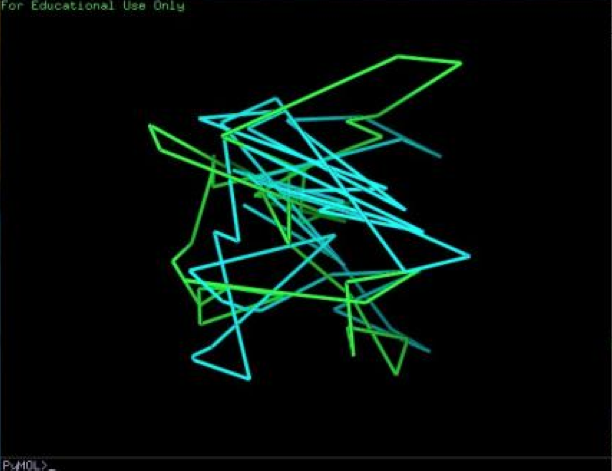
\includegraphics[scale=0.3]{Figure_1}
		\caption{The aligned embedding outcome of chromatin data from [6,7]}
	\end{figure*}
	\begin{figure*}[ht]\centering
		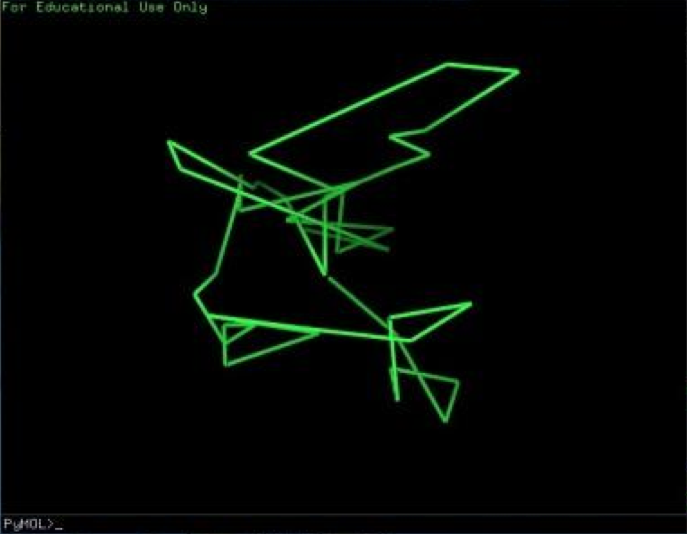
\includegraphics[scale=0.3]{Figure_2}
		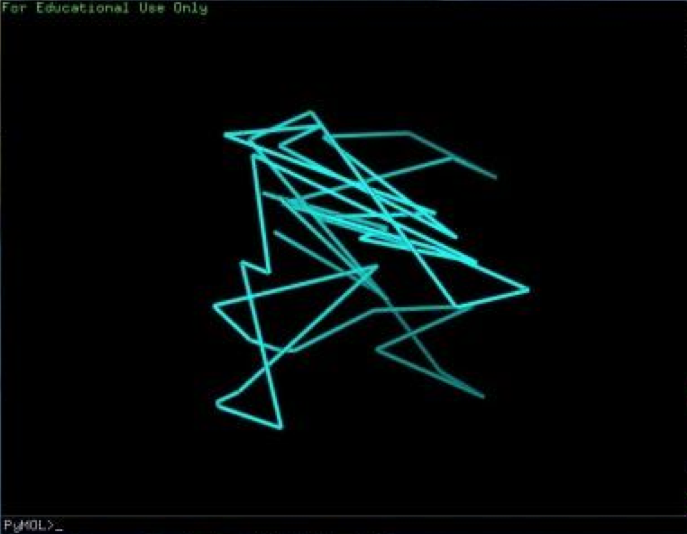
\includegraphics[scale=0.3]{Figure_3}
		\caption{Undifferentiated and Differentiated State of Figure 1}
	\end{figure*}

\subsection{Random data experiment}
	Please refer to Figure 4, 5 ,6 and 7.
	\begin{figure*}[ht]\centering
		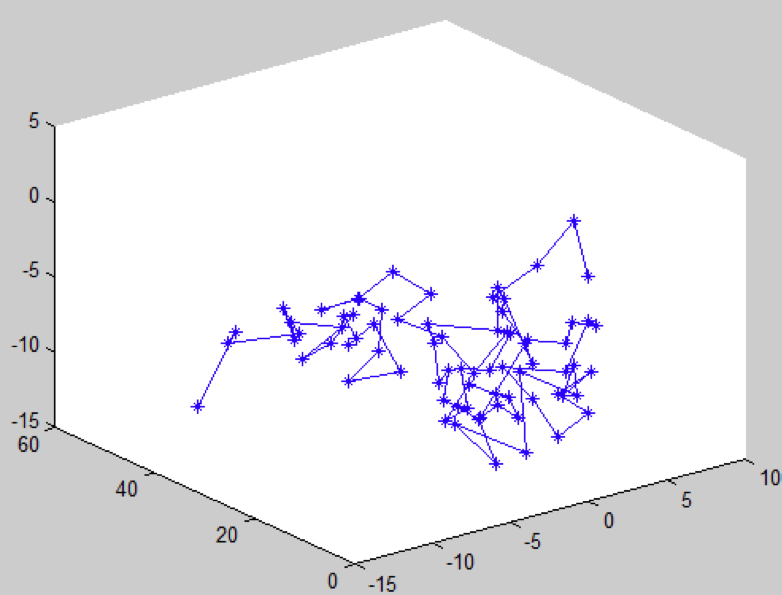
\includegraphics[scale=0.3]{Figure_4}
		\caption{Original structure generated randomly}
	\end{figure*}
	\begin{figure*}[ht]\centering
		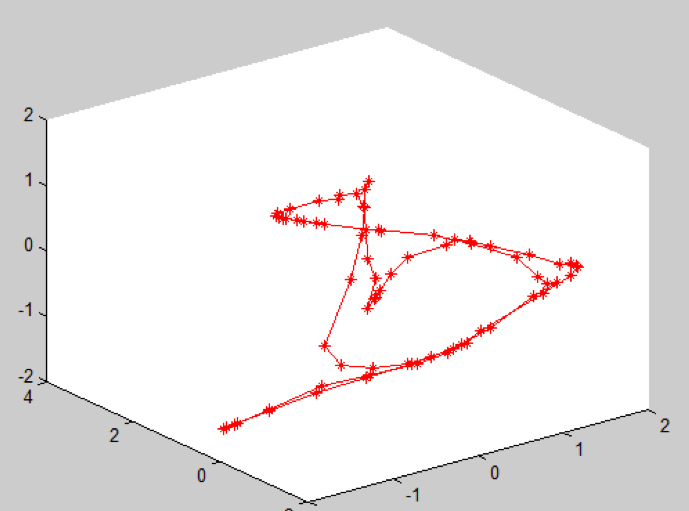
\includegraphics[scale=0.2]{Figure_5}
		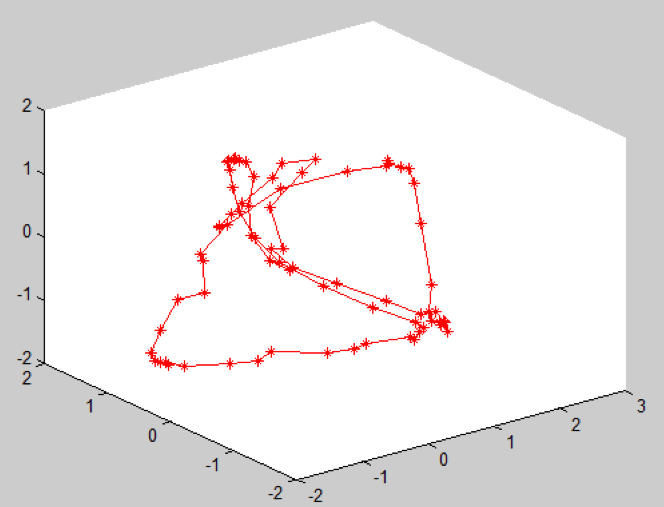
\includegraphics[scale=0.2]{Figure_6}
		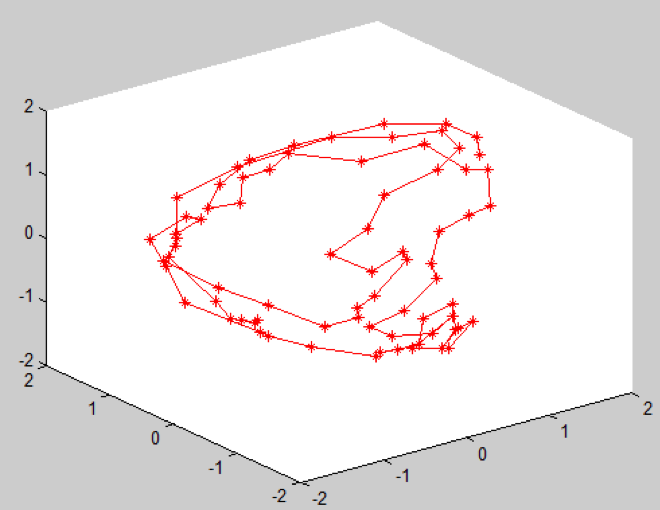
\includegraphics[scale=0.2]{Figure_7}
		\caption{Embedding with parameter $k = 3,7,15$}
	\end{figure*}

The outcome of our algorithms shows that our modified LLE algorithm performs poorly on reconstructing the 3D structure of randomly generated model. However, the implementation of the original algorithm, although having smaller RMSD on general, also leads to unsatisfying results. We believe that this indicates the unfeasibility of remodeling using LLE methods, and further analysis on the details of LLE with some attempts on explaining the reason are proposed.

%----------------------------------------------------------------------------------------
% MAJOR SECTION 4
%----------------------------------------------------------------------------------------

\section{Further Attempt to improve LLE}

%------------------------------------------------

\subsection{Possible reasons resulting failures}

The first reason involves with the IF information. In the data provided, we found that the IF information from one to its nearest points is not enough. It only contains IF from one to its nearest points, but IF from one neighbor to another is lost. The loss of IF information does not happen for this file only, but also all the other data downloaded. So we believe this is because of the restriction of detection techniques in biology. We are not able to resolve it.

The second reason is because of randomness of random structure. As we know, we generated the random data from a random walk. But for a chromatin structure, it should have some patterns inside, at least the energy is minimized. So it's not exactly random. We have thought of WL's method to decrease energy function by Gaussian perturbation, please refer to Simulated Annealing in WL's LLE-report. Following is the algorithm with input as of pairwise distance between each point, and output as of $Y_1,…,Y_N \in R^3$.

\begin{lstlisting}
Originally set the temperature T =10000, and the solution=[(0,0,0),(0,0,0),…,(0,0,0)]
Randomly take one point and add a vertex on it
Compute the difference d between the new solution and the old one
Repeat 10000 times:
	if (d<0):
		accept the new solution
	else:
		accept the new solution with probability e^(-d/T)
if the solution remains unchanged:
	return this solution
decrease the temperature to 0.92T
go back to step 2
\end{lstlisting}

However, WL's method is inapplicable when the number of points become large, which will cost $O(e^n)$.

Reason 3 is LLE doesn't work, or we didn't select good values for parameter k. This can be easily checked by plotting a graph between RMSD and parameter k.

%------------------------------------------------

\subsection{Analysis}

This time we will use real data, in order to get rid of the bias coming from Reason 2 discussed above. Secondly, we not only run the data for LLE but also for MDS, as a comparison. Thirdly, to avoid bias from Reason 3, we will run LLE with different k's. After running k with different values, we will then plot a line RMSD with respect to k, to see if there exist some k make LLE work better.

\subsubsection{1d3z.pdb}
Please refer to Figure 5,6 and 7.

\begin{figure*}[ht]\centering
	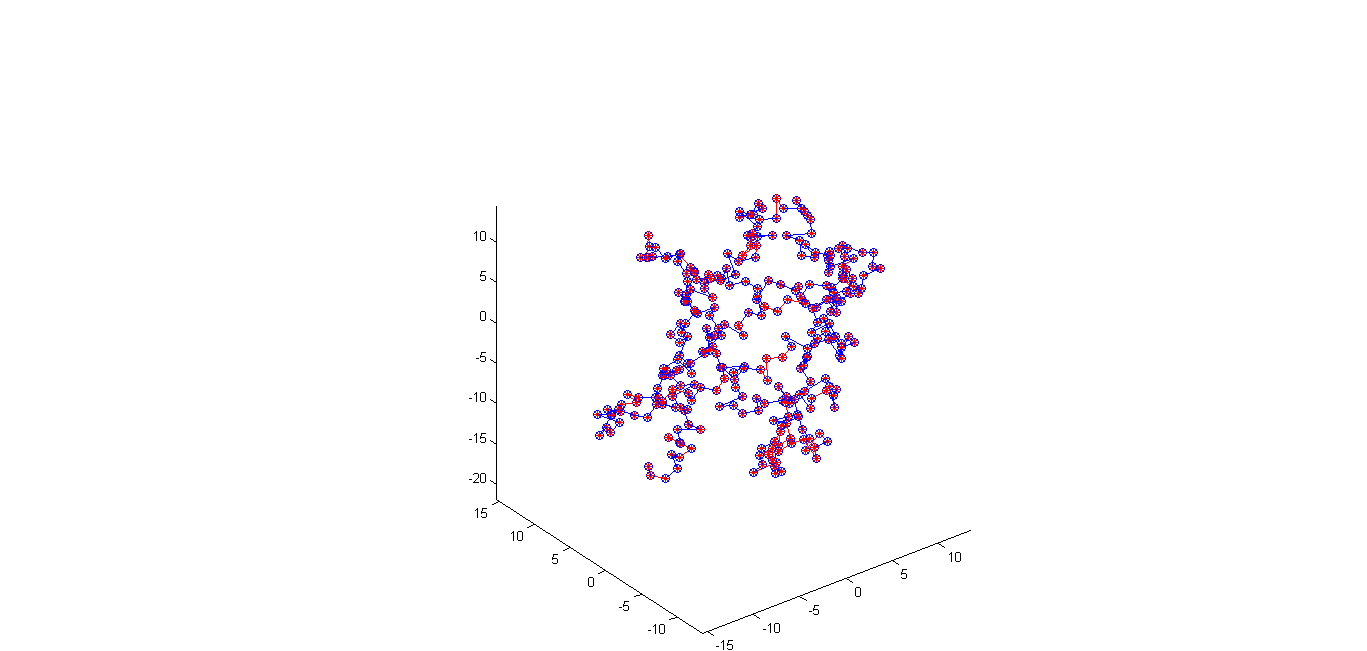
\includegraphics[scale=0.3]{fig01}
	\caption{MDS: RMSD = $2.2644 \times 10^{-5}$}
\end{figure*}

\begin{figure*}[ht]\centering
	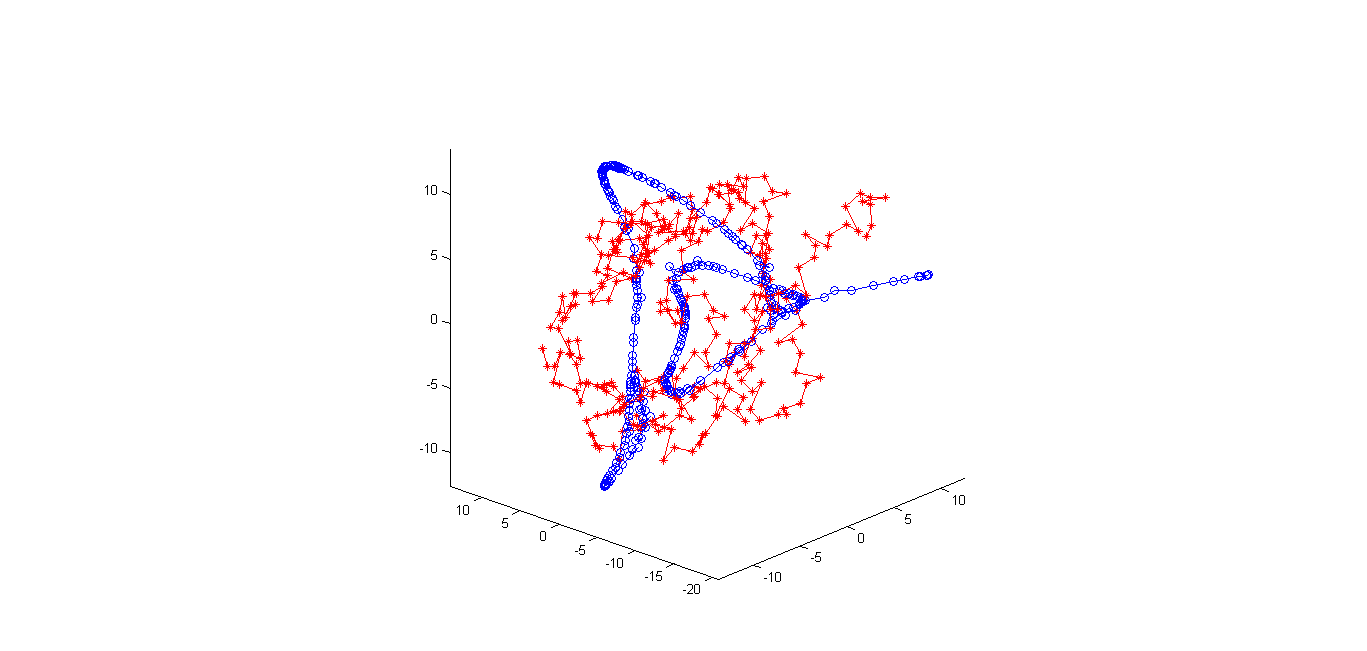
\includegraphics[scale=0.2]{fig1}
	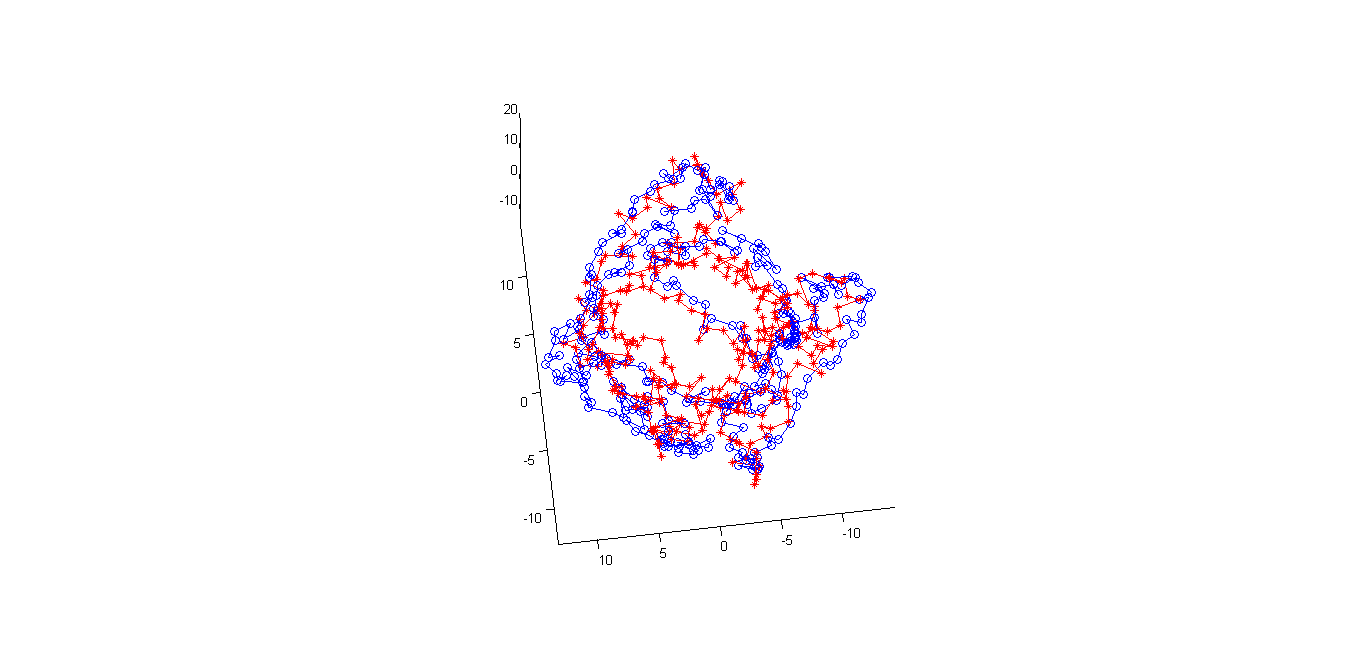
\includegraphics[scale=0.2]{fig6}
	\caption{LLE(7) \& LLE(250): RMSD = $6.0382$ \& $2.8712$}
\end{figure*}

\begin{figure*}[ht]\centering
	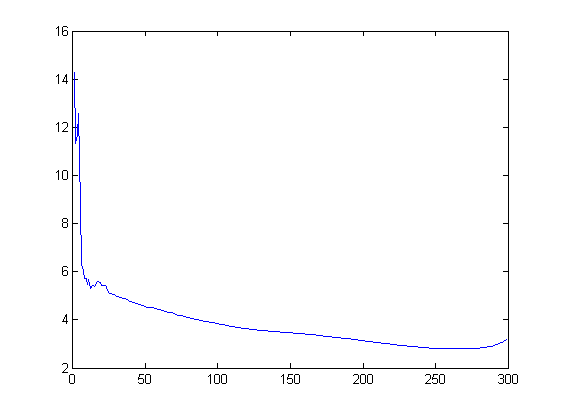
\includegraphics[scale=0.5]{fig4}
	\caption{LLE: RMSD - k from 1 to 299}
\end{figure*}

\subsubsection{1ubq.pdb}
Please refer to Figure 8,9 and 10.

\begin{figure*}[ht]\centering
	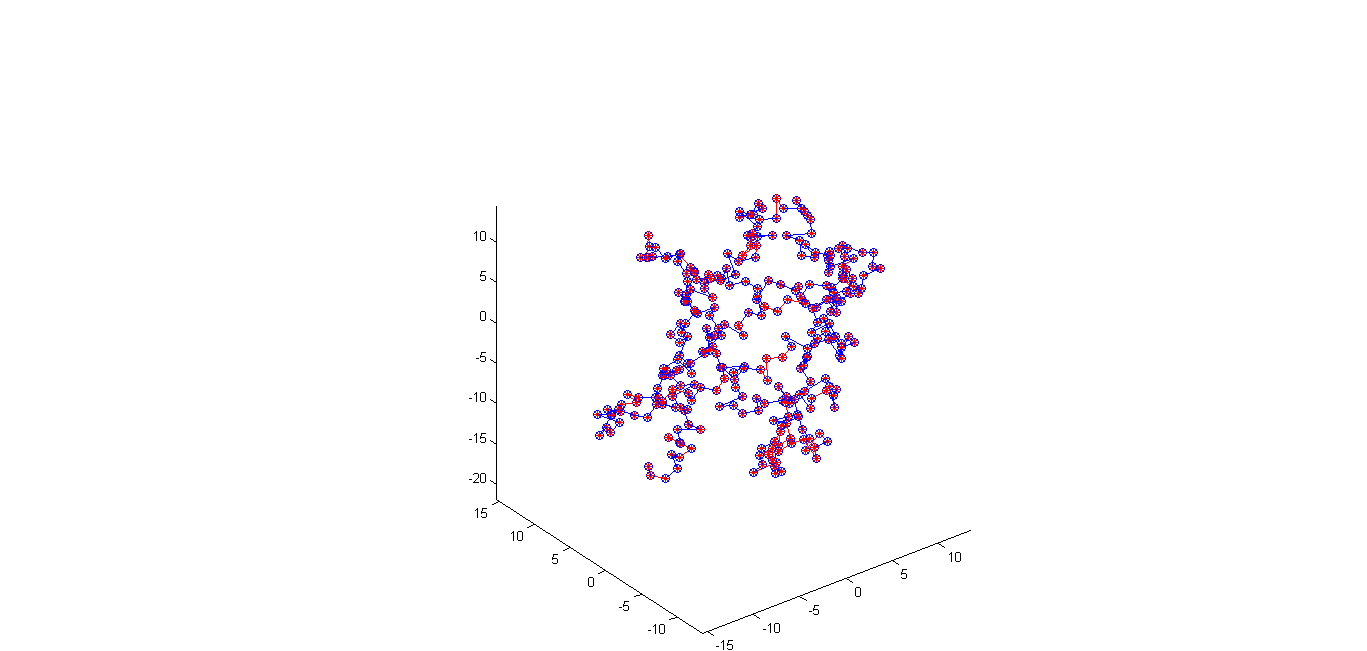
\includegraphics[width=\linewidth]{fig01}
	\caption{MDS experiment: RMSD = $6.2996 \times 10^{-5}$}
\end{figure*}

\begin{figure*}[ht]\centering
	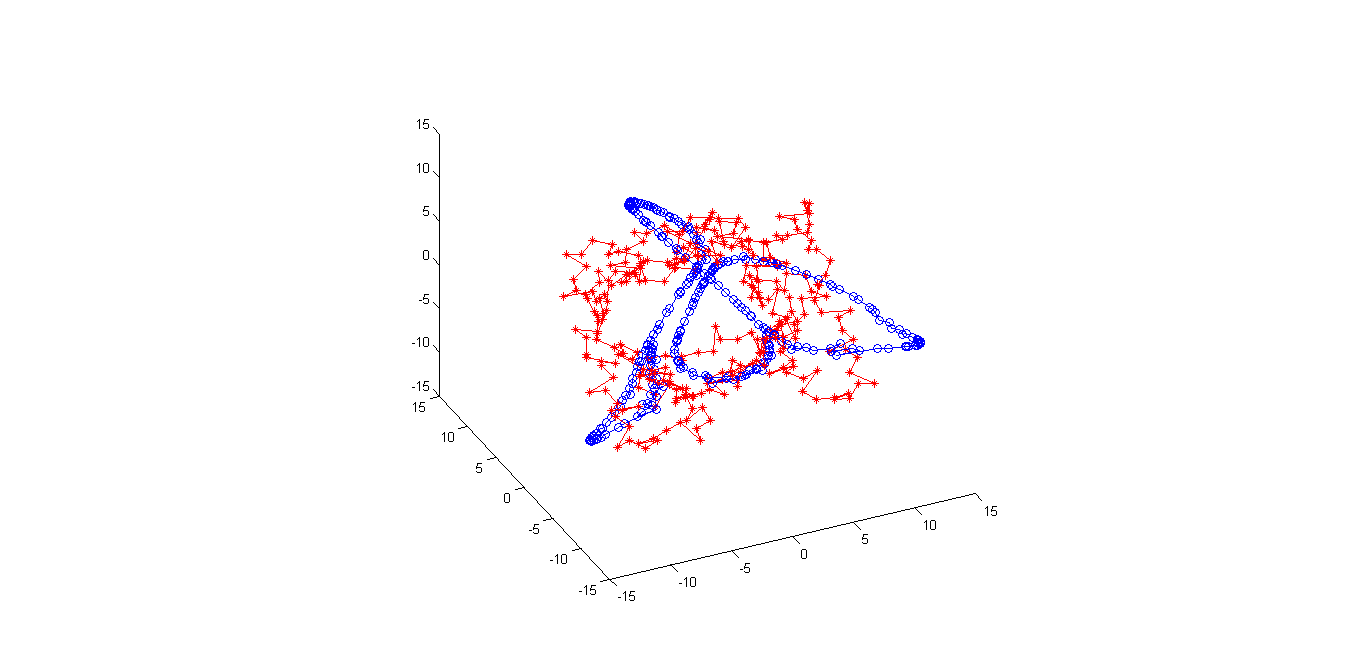
\includegraphics[scale=0.2]{fig2}
	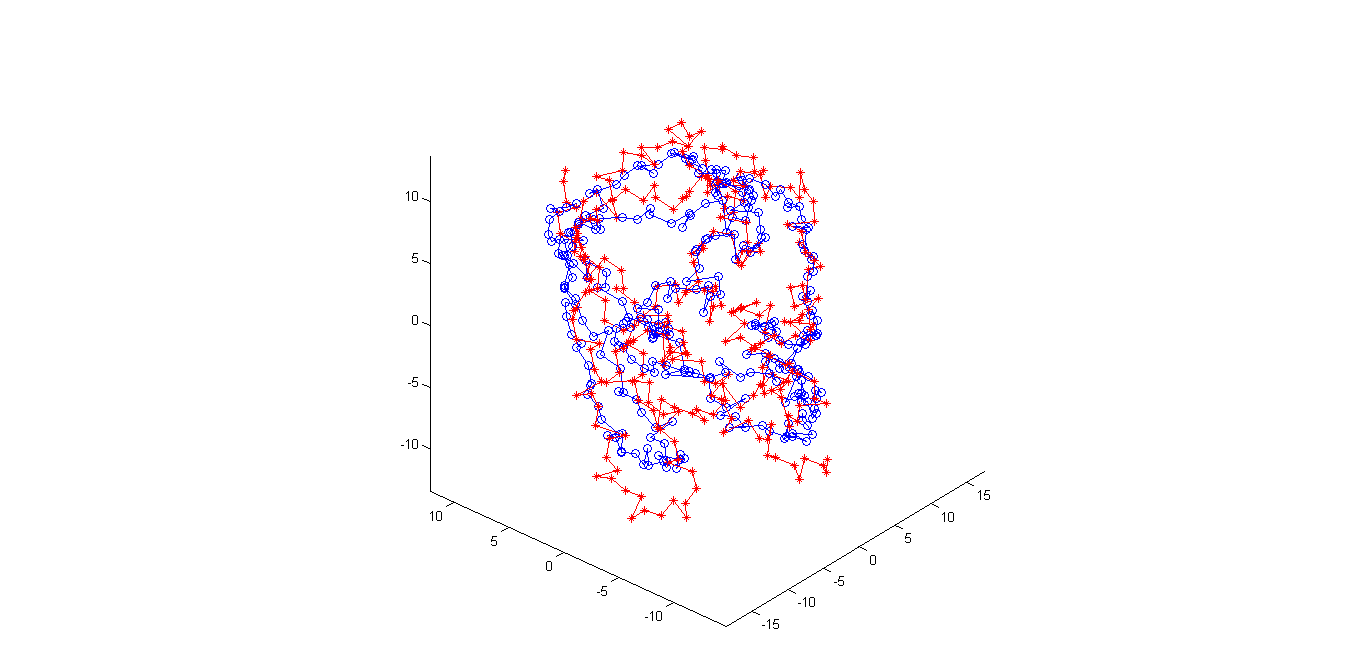
\includegraphics[scale=0.2]{fig5}
	\caption{LLE(7) \& LLE(250): RMSD = $5.3413$ \& $2.0217$}
\end{figure*}

\begin{figure*}[ht]\centering
	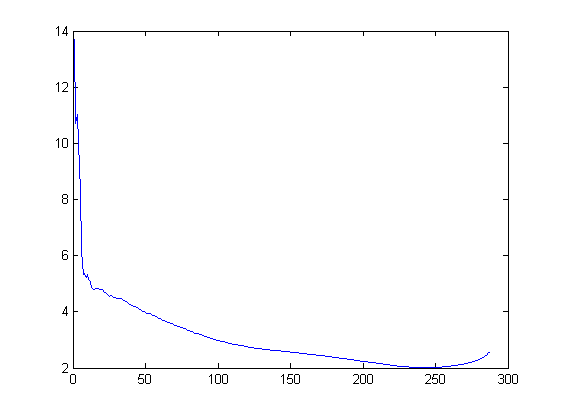
\includegraphics[scale=0.5]{fig3}
	\caption{LLE: RMSD - k from 1 to 287}
\end{figure*}

\subsubsection{1g7k.pdb}
Please refer to Figure 11, 12 and 13.

\begin{figure*}[ht]\centering
	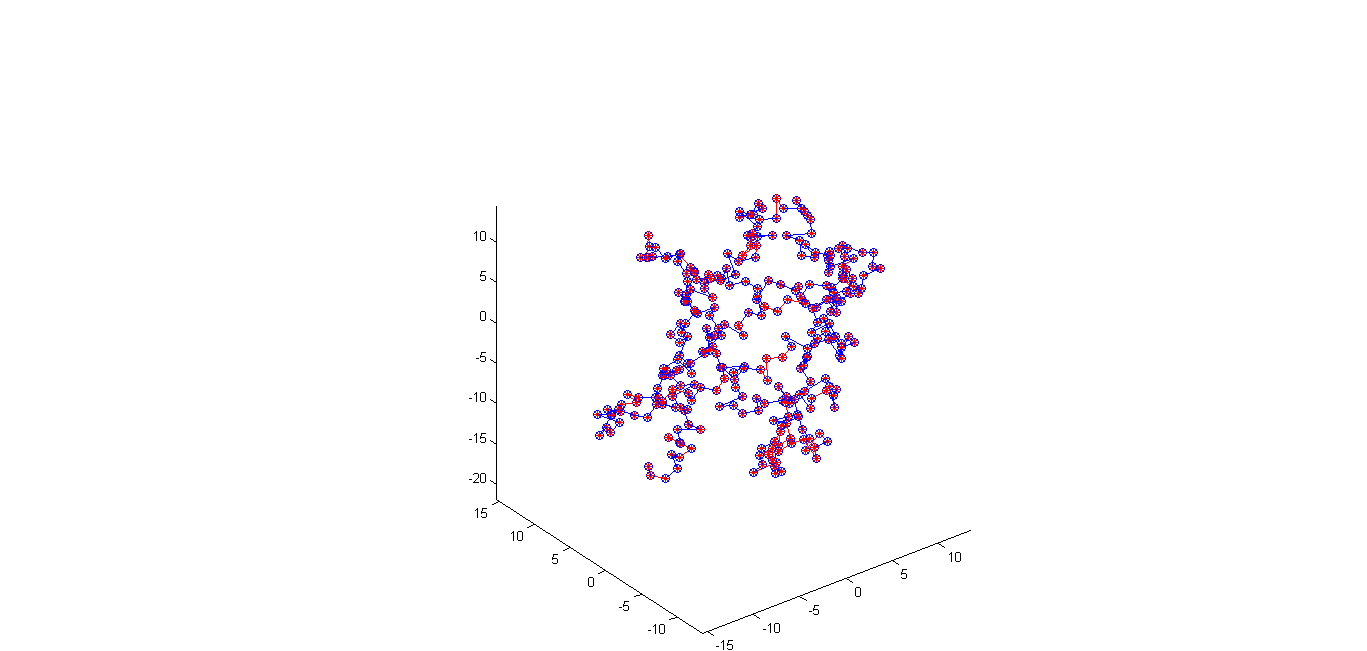
\includegraphics[width=\linewidth]{fig01}
	\caption{MDS experiment: RMSD = $3.3618 \times 10^{-5}$}
\end{figure*}

\begin{figure*}[ht]\centering
	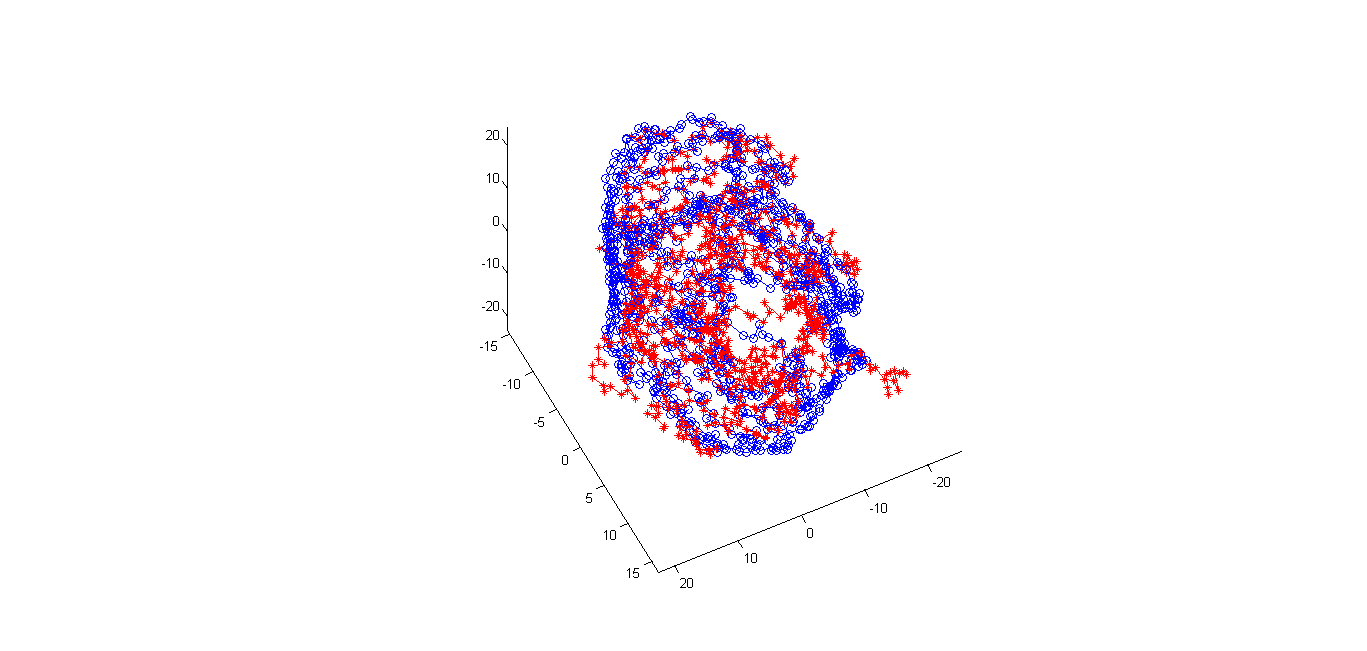
\includegraphics[scale=0.2]{fig8}
	\caption{LLE(790): RMSD = $4.3788$}
\end{figure*}

\begin{figure*}[ht]\centering
	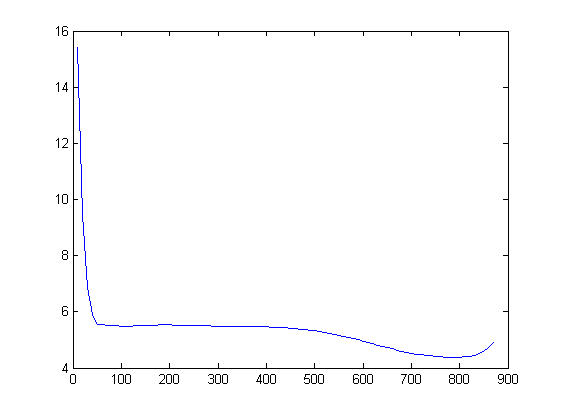
\includegraphics[scale=0.5]{fig7}
	\caption{LLE: RMSD - k from 1 to 287}
\end{figure*}

%----------------------------------------------------------------------------------------
%	CONCLUSION
%----------------------------------------------------------------------------------------

\section{Conclusion} % Major section

In the beginning, the LLE method fails to achieve the goal that reconstructs the structure from the simulated interaction frequency data, which has already been simplified to Euclidean distance data, even using whole pairwise distances without any noise. The result is far from our expectation, and we have analyzed the reasons for weeks, including discussion with Zhengyu Wang and Lingyu Wei. Fortunately, we replace former experiment using random data by real data, and test it with much larger parameter k, find it seems possible to make LLE work well.

Lingyu Wei has introduced Simulated Annealing approach to optimize complicated objects. It works well but has time inefficiency. In our project, we made use of it and utilized to transform random structure data to more reasonable low energy structure data. The goal is just to minimize a function of points which suffers a penalty when the distance is different from the input. However because of its large time complexity, it is inapplicable in reality when the number gets much larger.

Comparing MDS and LLE, though we find LLE can work well within some range, but still performs much worse than MDS. After doing all these analysis, given data of matrix implying relationship between each two points, we generate structures of them. However we don't have the real structure of those data, so it's just a practice shown from Figure 14 to Figure 18. Please advisor help check its correctness if got their structure.

\begin{figure*}[ht]\centering
	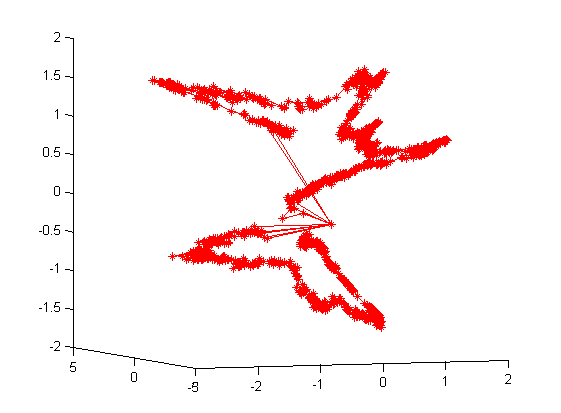
\includegraphics[scale=0.5]{fig001}
	\caption{Structure of uij.chr20.csv}
\end{figure*}

\begin{figure*}[ht]\centering
	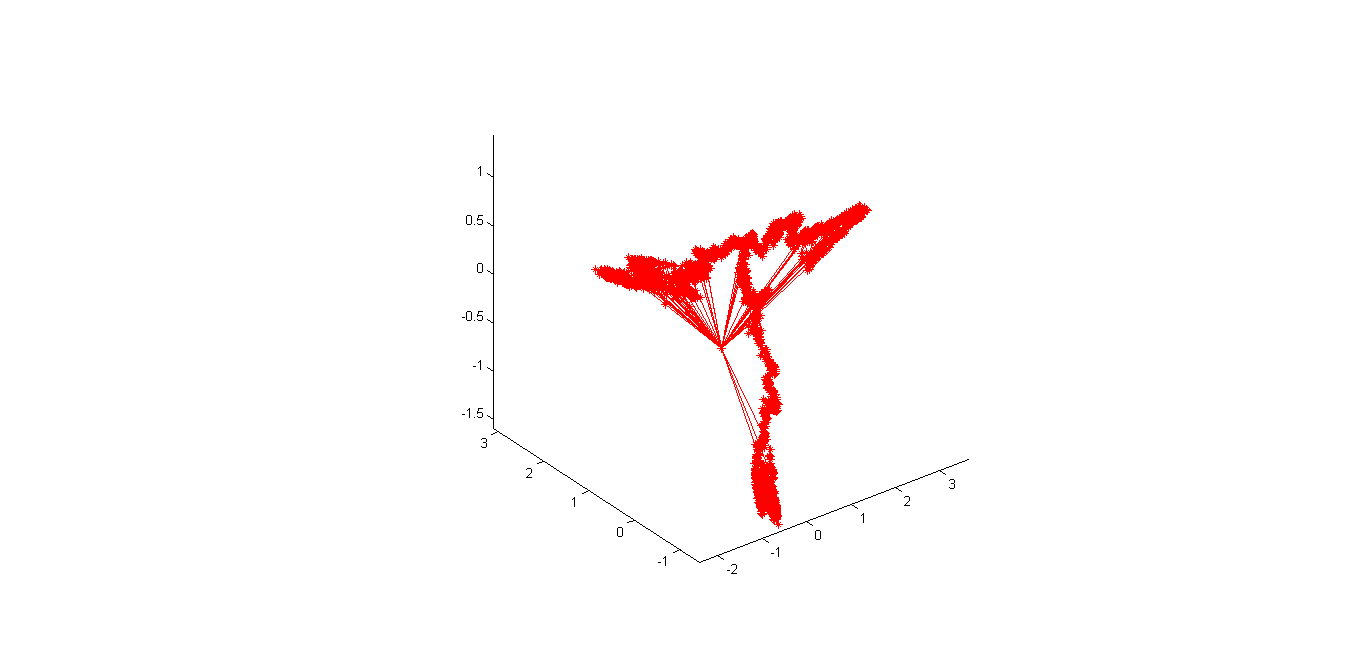
\includegraphics[scale=0.5]{fig002}
	\caption{Structure of uij.chr23.csv}
\end{figure*}

\begin{figure*}[ht]\centering
	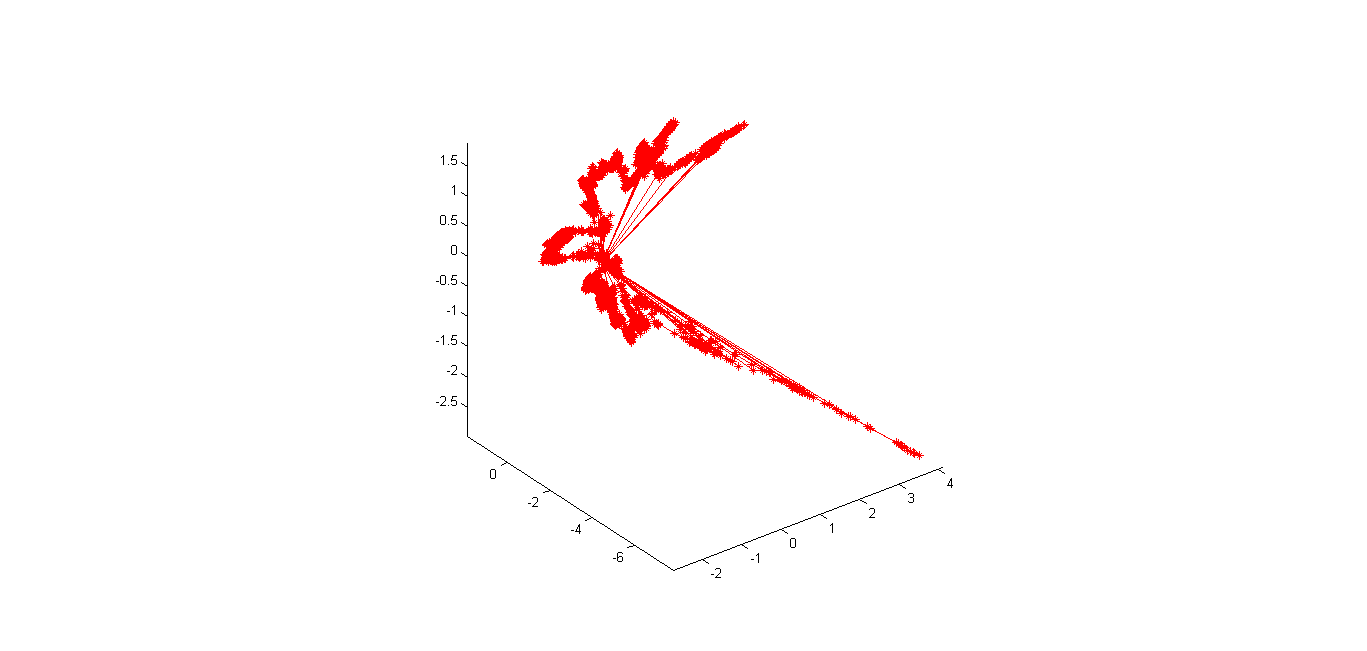
\includegraphics[scale=0.5]{fig003}
	\caption{Structure of uij.chr7.csv}
\end{figure*}

\begin{figure*}[ht]\centering
	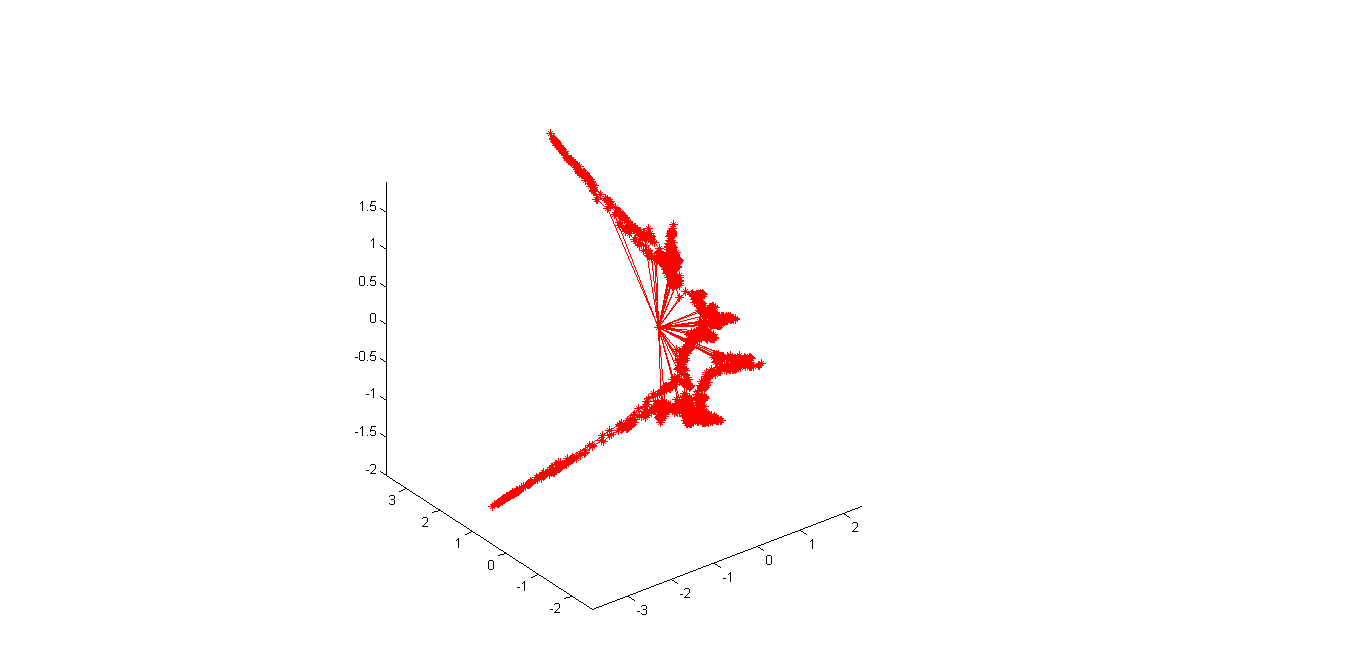
\includegraphics[scale=0.5]{fig004}
	\caption{Structure of uij.chr17.csv}
\end{figure*}

\begin{figure*}[ht]\centering
	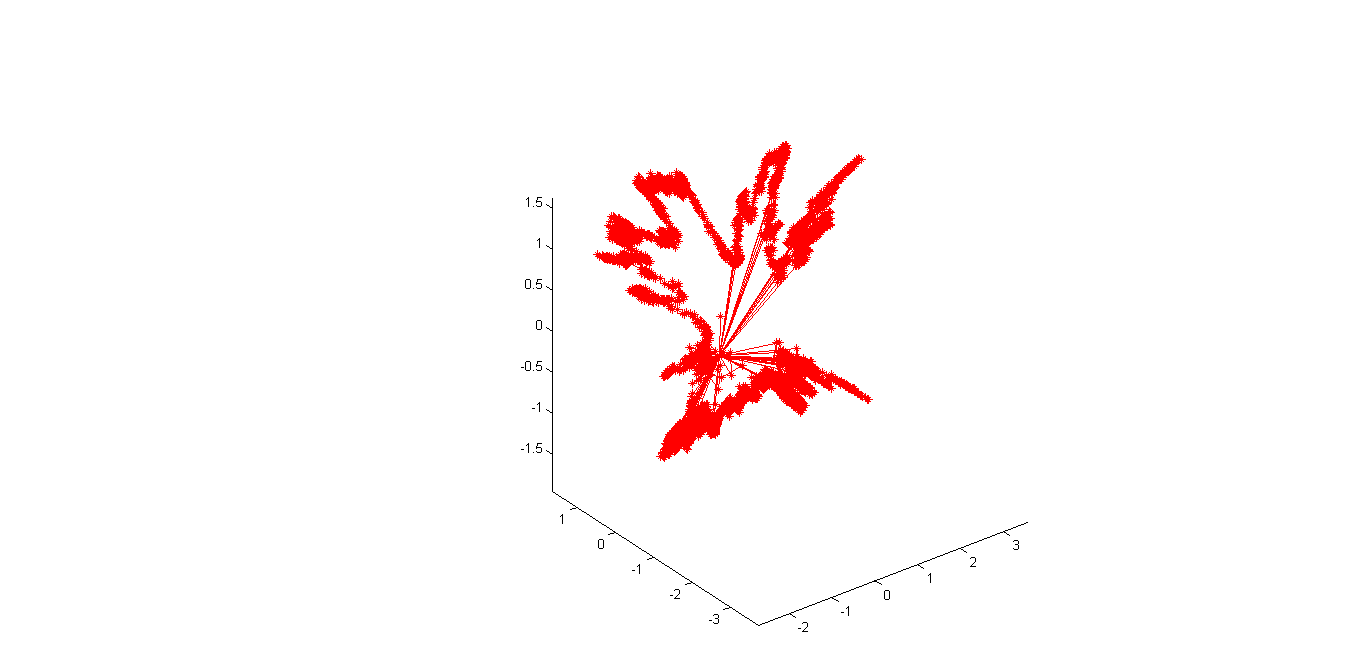
\includegraphics[scale=0.5]{fig005}
	\caption{Structure of uij.chr1.csv}
\end{figure*}

%----------------------------------------------------------------------------------------
%	BIBLIOGRAPHY
%----------------------------------------------------------------------------------------

\begin{thebibliography}{99} % Bibliography - this is intentionally simple in this template

\bibitem[1]{1}
L. Saul and S. Roweis, An Introduction to Locally Linear Embedding.
 
 \bibitem[2]{2}
S. Roweis and L. Saul, Nonlinear Dimensionality Reduction by Locally Linear Embedding. Science 290,pp.2323-2326 (2000)

\bibitem[3]{3}
\href{http://chromosome.sdsc.edu/mouse/hi-c/index.html}{\textcolor{blue}{Chromosome}}

 \bibitem[4]{4}
\href{http://www.cs.nyu.edu/~roweis/lle/}{\textcolor{blue}{CS NYU}}

 \bibitem[5]{5}
\href{http://en.wikipedia.org/wiki/Nonlinear_dimensionality_reduction}{\textcolor{blue}{Wiki Nonlinear dimensionality reduction}}

 \bibitem[6]{6}
Fraser J, Rousseau M, Shenker S, Ferraiuolo MA, Hayashizaki Y, Blanchette M, Dostie J.,Chromatin Conformation Signatures of Cellular Differentiation. Genome Biol. 2009;10(4):R37

 \bibitem[7]{7}
Rousseau M, Fraser J, Ferraiuolo MA, Dostie J, Blanchette M. Three-Dimensional Modeling of Chromatin Structure from Interaction Frequency Data Using Markov Chain Monte Carlo Sampling.BMC Bioinformatics. 2011.

 \bibitem[8]{8}
Jianyang Zeng, Suggested Topics for Final Project, Computational Biology (2014 Spring).

 \bibitem[9]{9}
\href{http://www.cse.wustl.edu/~kilian/research/manifold/manifold.html}{\textcolor{blue}{Manifold Learning}}

\end{thebibliography}

%----------------------------------------------------------------------------------------

\end{document}